% !TEX root = ../Thesis.tex
\begin{document}
\documentclass[Thesis.tex]{subfiles}
\chapter{Recommender System}
\label{ch:recommender_system}

The main objective of this thesis is to build a prototypical recommender system for the physician letters and assess its quality. We do so based on the document embedding methods introduced in chapters \ref{ch:dataset cleansing} and \ref{ch:infpres}. Once documents are embedded in a vector space similarities between documents $d_1$ and $d_2$ can be computed as the cosine similarity of the corresponding vectors $\rm{sim}_{\cos}(\textbf{v}_{d_1}, \textbf{v}_{d_2})$. To find the letters, that are most relevant, given a reference letter, that we are currently interested in, we compute the similarity of the reference letter to all other letters in the database. Thereby we get a ranking of all other letters, given the reference letter. The "best" fitting letter or the letter with rank one is considered the most relevant according to the algorithm. The $n$ most relevant letters are the ones on the $n$ highest ranks or the $n$ letters with highest cosine similarity to the current reference letter. They can be retrieved from the database and presented to a user.

\section{Fine-tuning}
Based on the cosine similarity between vectors of the corresponding texts all document embedding methods can in principle be used as a base for the recommender system. To find out which hyperparameters and which embedding method works best we use supervised similarity information. The most desirable information is an expert rating of similarity between letter pairs. As this information is expensive to come by, because experts working hours are expensive, we use a different, easier acquirable dataset for the task of fine-tuning. This data consists of a grouping of 135 of the letters into 50 non-overlapping groups of similar patients done by an expert. Some groups only contain a single patient (if he/she was dissimilar to all others), some contain several and the average group consists of 2.7 patients. This grouping is not equivalent to a correct measure of similarity, but we can still use it as an approximate measure of similarity to tune our algorithm. Thereby letters from the same group are considered similar and letters from different groups are considered dissimilar. One measure of goodness for a real recommender system is how often the system ranks the truly similar letters into the top $n$. I.e. given one reference letter, are the similar letters of the grouping dataset considered to be among the top $n$ most relevant by the recommender system.  We call this the top-n measure. This measure, however, does not take all available information into account. Say we specify $n=5$, the top-n measure gives the same score, if a truly similar letter is ranked to be the 6th most similar or the least similar of all. A measure that assigns a higher score in the first situation than in the second would be preferable for the fine-tuning of the algorithm. We therefore develop a continuous measure, that assigns a score from the interval $[0,1]$ for all possible ranking situations. A score of 1 is given, if the truly similar letters occupy the foremost positions, a score of 0, if the truly similar letters occupy the last positions, a score of 0.5, if the truly similars occupy the positions in the centre. A score of 0.5 is expected, if the algorithm sorted the letters by chance.

Based on the continous measure we first do hyperparameter tuning for the embedding methods as applicable. Afterwards we select the best performing embedding method the same way. Table \ref{table:continuous_measure} shows the scores obtained by each embedding method. Generally the performance is high above chance level. It is noteworthy that the simple and hyperparameterless tf-idf method outperforms all other methods including LDA and the recent and hard-to-tune paragraph vector. We therefore choose tf-idf as the embedding method for the recommender system. 

There are good reasons that tf-idf works so well for our problem. It is plausible that the main features for human similarity judgments of letter pairs are based on the diagnosis of the patients. The diagnosis and diseases words are features that the tf-idf method will judge as very important, as they appear only in few documents overall. An additional problem, however, is that of different spellings of the same disease. Consider for example the disease "chronic lymphocytic leukemia". Spellings range from "CLL" over "B-CLL" to "chronic-lymphocytic-leukemia". All these spellings are regarded by all our models as separate entities. However, the tf-idf vectors are still useful document embeddings, as the overall word statistics still differ depending on the diagnosis. Words describing medication for leukemia for example are still present in all letters of patients with CLL. These medication words, however, are again present only in few documents overall and are thereby considered more important features by the tf-idf method.
\begin{table}
	\begin{tabular}{|c||c|c|c|c|c|}
		\hline 
		Embedding Method & BOW & TF-IDF & LSA & LDA  & Para2Vec\tabularnewline
		\hline 
		\hline 
		Continous Measure Score & 0.794 & \underline{0.870} & 0.868 & 0.634 & 0.830\tabularnewline
		\hline 
	\end{tabular}
	\caption{Performance of different embedding methods (with tuned hyperparameters) on the grouping dataset evaluated with the continous measure.}
	\label{table:continuous_measure}
\end{table}



\section{Recommendation Quality---Experimental Setup}
Having fine-tuned the recommendation procedure as described above the next step consists of assessing the quality of the recommendation. We test this quality in a psychological experiment. To this end we probe the similarity ratings that subjects give to pairs of letters and compare them to the similarity measure of our algorithm.

We construct an experiment with 32 ``trials'', in which subjects have to compare letter pairs for similarity. More precisely that means we select 32 letters as ``reference letters'' out of our database and let subjects rate the similarity of these 32 reference letters to five other letters each. Thereby we gain ratings for 160 letter pairs. 16 of the reference letters have a follow-up letter in our database. Trials with this kind of reference letter are called ``follow-up trials'' and letter pairs of follow-ups are called ``follow-up pairs''. The other 16 reference letters are selected randomly among the letters without follow-ups present in our dataset. The five letters that are compared to one reference letter are called the comparison letters. Four of them are selected based on the cosine similarity between the reference letter and all other letters. These four are the ones with highest cosine similarity to the reference letter according to our algorithm. That means they are the best matches to the reference letter according to our algorithm---or equivalently, they are ranked on places one to four given a reference letter. The fifth comparison letter is randomly selected among all other letters and then fixed. Subjects are presented with one reference and one comparison letter at a time. After rating their similarity they are presented with the next comparison letter. Once a trial is done, i.e. five comparison letters are rated, the next reference letter is presented. The order of the reference and comparison letters is random, but fixed. Subjects are forced to give a rating in the range of 1 (very dissimilar) to 7 (very similar) for each letter pair.% See figure \ref{fig:webexperiment} for a screenshot of the website on which the subjects perform the experiment.

We design the experiment such that the first trial is a follow-up trial and the second one is a non-follow-up trial. Thereby we ensure that subjects can adjust for the upper similarity bound of having to compare letters of the same patient. These two trials are excluded for the later analysis. We have six subjects performing the experiment, four experts (oncologists with at least five years of practical experience) and two novices (medical students more than halfway through their study course).


%\begin{figure}
%	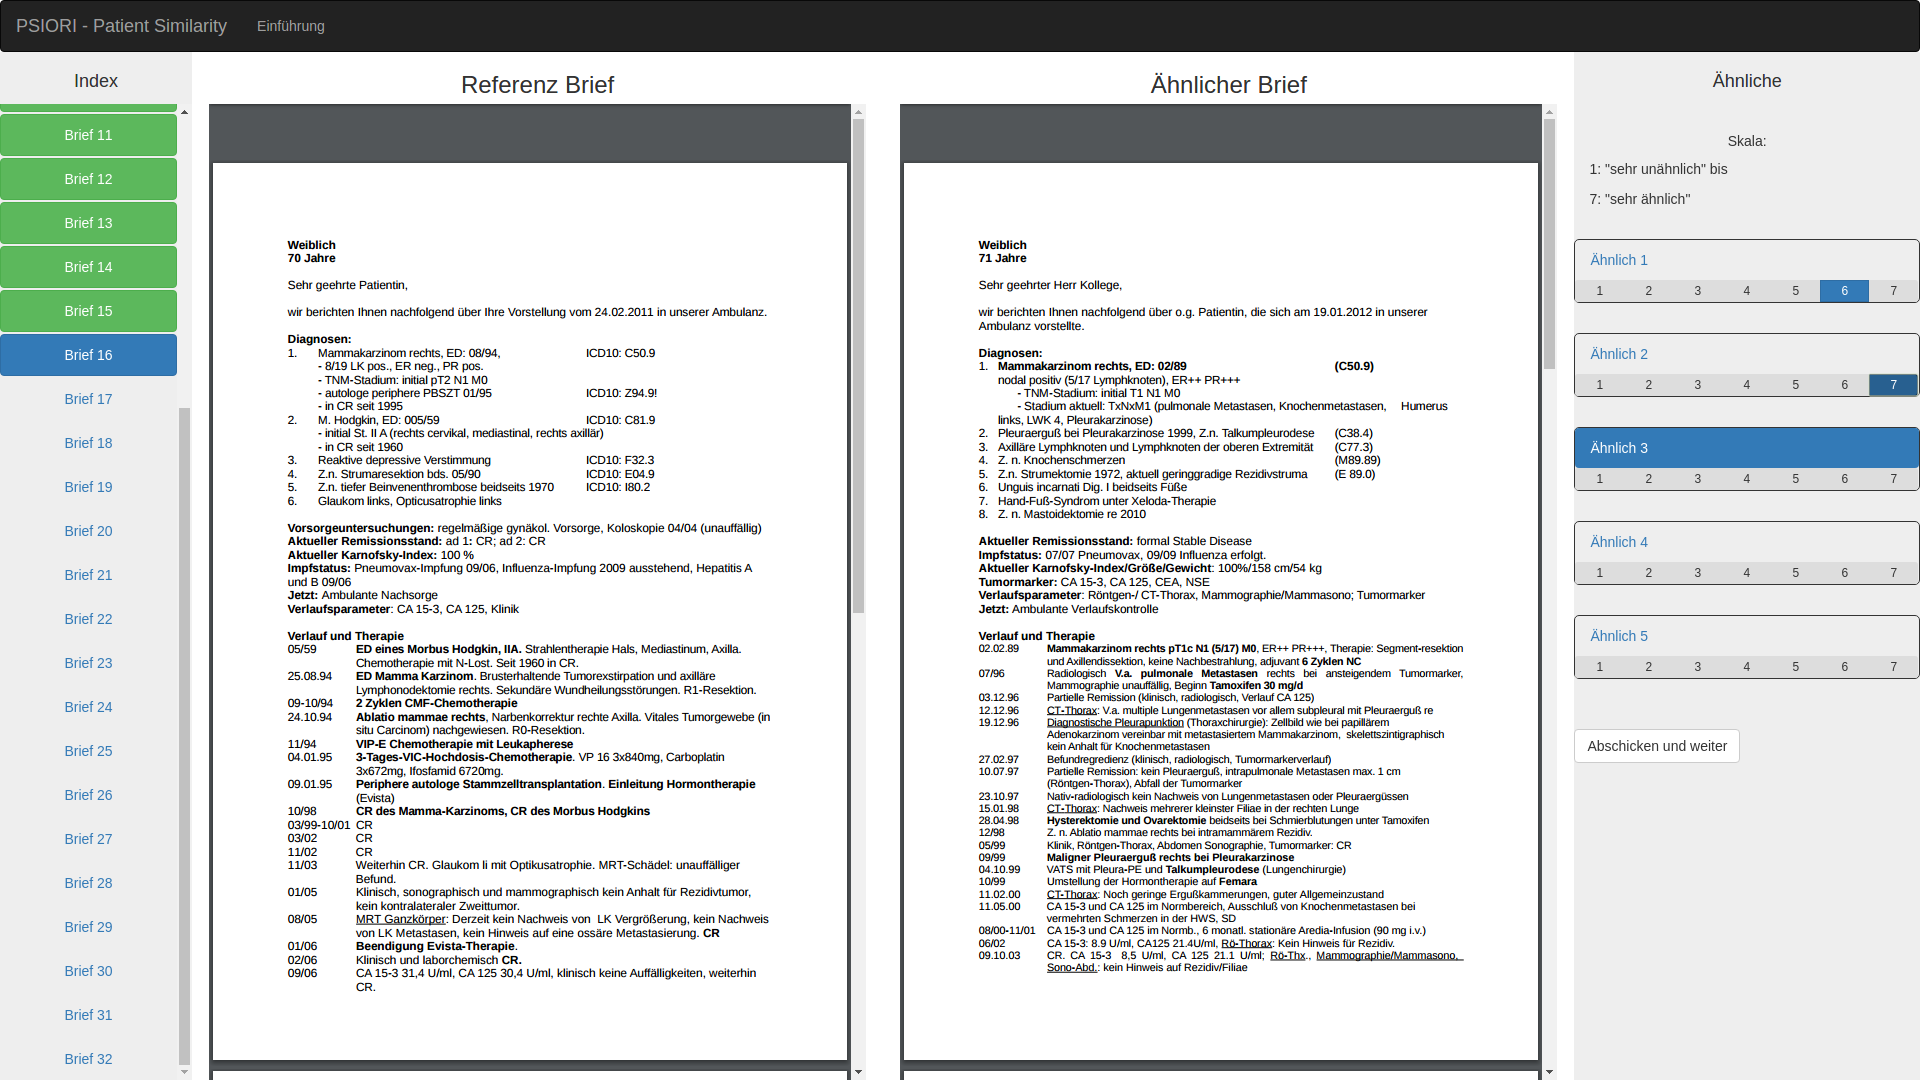
\includegraphics[width=\linewidth]{figures/webexperiment_screenshot2}
%	\caption{Screenshot of the website view during the experiment.}
%	\label{fig:webexperiment}
%\end{figure}



%We probe the similarity ratings that subjects give to pairs of letters and compare them to the similarity measure of our algorithm. We select 32 letters out of our database, 16 of them have a follow-up letter in our database, the other 16 are randomly selected among the ones without follow-up letter. We take these 32 as reference letters and select to each of them five other, so called comparison letters, with which they will be compared for similarity. Four of these five are the ones with highest cosine similarity to the reference letter as computed with our algorithm. The fifth is randomly selected and then fixed. Subjects are presented with a reference letter and the five comparison letters in a random, but fixed sequence. They are forced to give a rating for each pair in the range of 1 (very dissimilar) to 7 (very similar) and can then move on to the next reference letter. See figure \ref{fig:webexperiment} for a screens hot of the website on which the subjects perform the experiment. We ensure that among the first two reference letters is one follow-up reference letter and one non-follow-up reference letter. This way subjects can adjust for the upper similarity bound of having a letter pair with both letters from the same patient. In total we obtain ratings for 160 letter pairs from each subject. However, the rating data for the first two reference letters is discarded for the later analysis, leaving 150 letter pairs for evaluation. Six subjects perform our experiment, four experts (oncologists with at least five years of practical experience) and two novices (medical students more than halfway through their study course).



\section{Recommendation Quality---Results}

\subsection*{Inter-Rater Agreement}

We first analyze the inter-rater agreement among subjects. We believe it is not trivial for them to rate physician letter pairs for similarity as it is not directly clear along which dimension similarity is to be judged, a problem well known from the cognitive science literature \citep{Medin1993}. One might for example judge similarity based on diagnosis or based on therapy. We also believe that experts and novices (or students) base their judgments on different features. Experts generally have higher agreement when categorizing stimuli, than novices do, and usually use more abstract, less accessible features \citep{Chi1981, Linhares2007, Leon-Villagra2013}. In line with these results we find that the inter-rater agreement is higher among the experts than among the students (expert agreement: 0.83; student agreement: 0.73). We measure this agreement with the spearman rank correlation coefficient, that produces a number between -1 (perfect anti-correlation) and 1 (perfect correlation). Spearman's coefficient is used instead of the often used cohen's kappa coefficient, because the former can deal with ordinal data, whereas the latter can only deal with nominal data \citep{Spearman1904, Cohen1960}. Our number of subjects is quite low for concluding that students rate letter pairs worse than experts. Still as our findings are in line with well established research, we discard the student rating data for further analysis. 

Note that for the following analyses we exclude data of follow-up pairs, except where explicitly stated otherwise. Subjects rate the similarity of these pairs very highly and almost any information retrieval system will find them to be similar. Thereby they would improve positive correlation statistics in our analysis, although retrieving them is useless in practice. We will show later that our recommender can easily distinguish them from normal pairs.

\subsection*{Ranking and Subject Ratings}

The first analysis concerning our recommender system asks the question whether the recommendations are better than chance. Therefore we compare the average subject rating of the comparison letter with highest cosine similarity to a reference letter (i.e. the "best fitting" letter or the letter with rank one, according to our algorithm) to the rating of the randomly chosen comparison letter for each trial. Figure \ref{fig:best_vs_random} shows the means and standard deviations of the average rating that subjects gave to the "best" and randomly selected letters. One sees that letter pairs with highest cosine similarity are rated higher than the randomly chosen ones. However, both groups show a high standard deviation. For the group of letters selected by our algorithm this might be caused the following way. Often the algorithm can find a good match and the rating of subjects will be high. However, sometimes a good match is just not found and the rating is low. This can happen due to several reasons. First our algorithm might just not find the fitting letter from our database. But second our small dataset might just not include a fitting letter to a reference letter. In this case the best letter we can find in principle is still rated low by subjects. We will address this problem further, when discussing the connection between letter pair cosine similarity and subject rating more thoroughly. 

Additionally we estimate the effect size of using the "best" compared to the random letter. This is done through bootstrapping \citep{Efron1979}. Bootstrapping is a procedure in which many random resamples of the dataset are computed. If our collected dataset represents the true distribution of ratings of "best" and random letter pairs well enough, then the resamples are to our sample as our sample is to the true distribution. Thereby the differences in mean of the resamples give an estimate of the differences in mean, when collecting many samples from the real distribution. We take 100.000 resamples with replacement from our data and compute the difference in mean for every one of them. The distribution of the differences in resample means can be seen in figure \ref{fig:bootstrap_diff}. In the figure one can also see that the 95\% confidence interval for the improvement of the average subject rating, when using the "best" letter computed with our algorithm instead of a random one, starts at 1.2 and goes to 2.7 with a mean improvement of 1.9 on the rating scale from 1 to 7.

\begin{figure}
	\centering
	\begin{subfigure}[b]{0.33\textwidth}
		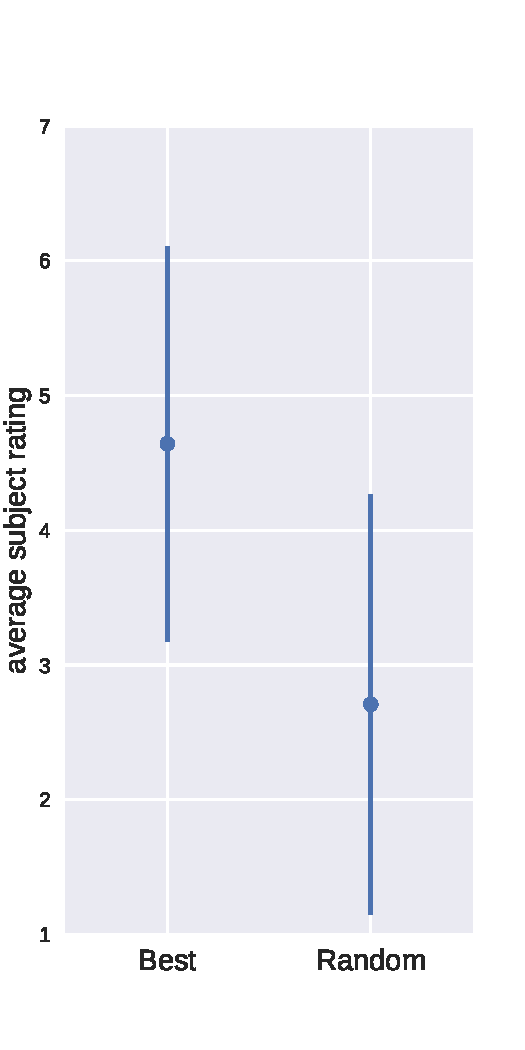
\includegraphics[width=\textwidth, valign=t]{figures/best_vs_random}
		\caption{}
		\label{fig:best_vs_random}
	\end{subfigure}
	\hfill
	\begin{subfigure}[b]{0.66\textwidth}
		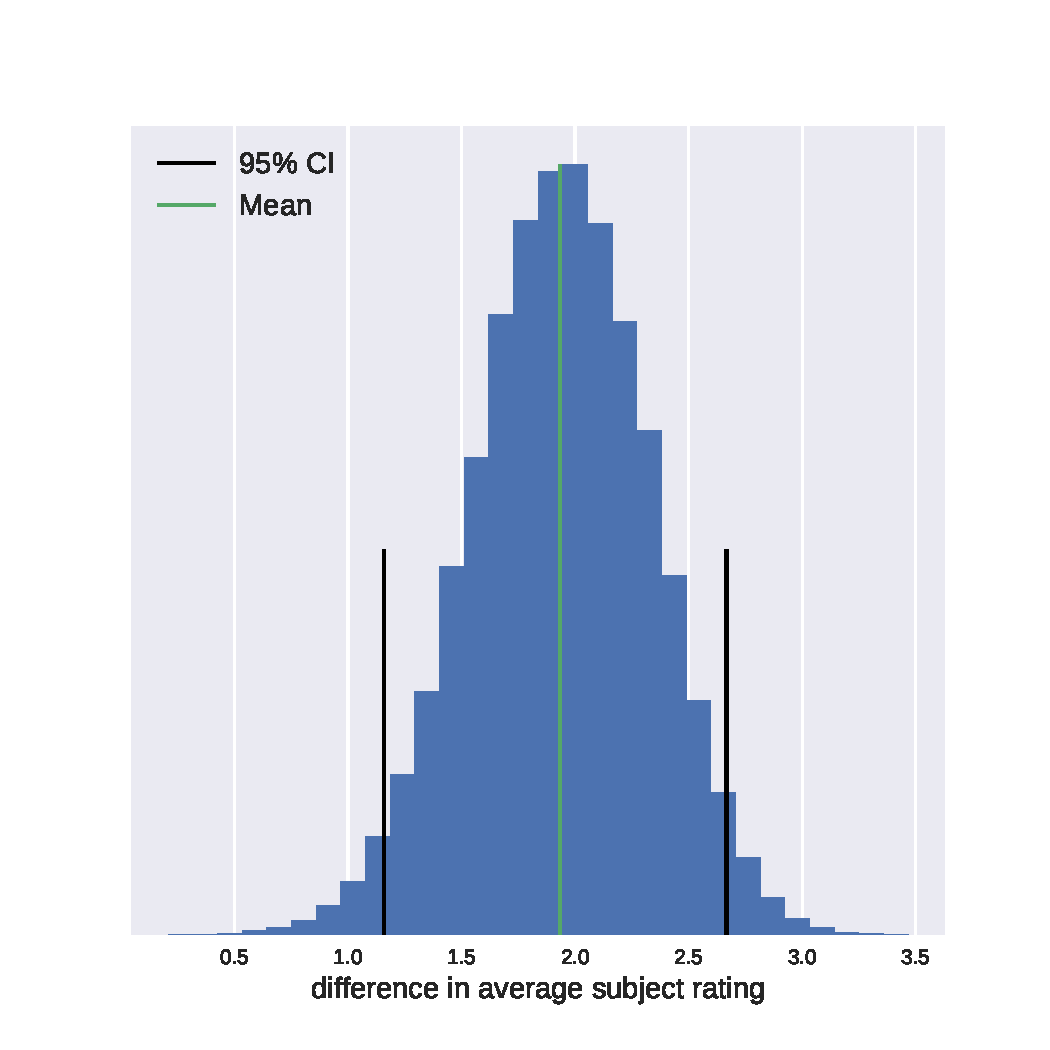
\includegraphics[width=\textwidth, valign=t]{figures/mean_diff_best_random}
		\caption{}
		\label{fig:bootstrap_diff}
	\end{subfigure}
	\caption{\textbf{(a):} Means and standard deviations of averaged subject ratings for the best letters chosen by our algorithm and randomly chosen letters.
		\textbf{(b):} Histogram of the differences in the means of averaged subject ratings of the two groups for 100.000 bootstrap resampled datasets. Black: 95\% Confidence Interval, Green: Mean}	
\end{figure}

\subsection*{Cosine Similarity and Subject Ratings}
\begin{figure}
	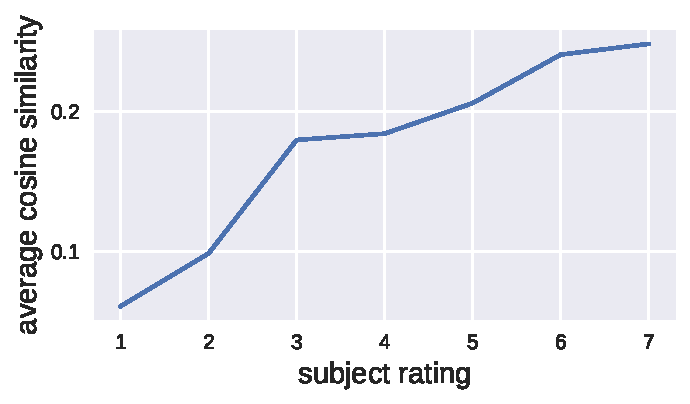
\includegraphics[width=\linewidth]{figures/rating_vs_sim_mean}
	\caption{Averaged cosine similarity of all letter pairs that were rated into one of the seven possible rating categories.}
	\label{fig:rating_vs_sim}
\end{figure}


After analyzing whether ranking letter pairs with our algorithm works better than chance, we analyze the relationship of the cosine similarity and the average subject ratings of letter pairs more directly. We visualize the mean cosine similarity, that our algorithm assigns to pairs, as a function of the subject rating in figure \ref{fig:rating_vs_sim}. The data shows a positive, close to linear correlation (pearson correlation: 0.93) of those two variables, suggesting that our recommendation method captures at least some aspects of perceived similarity.

Next we analyze the relationship of the cosine similarity and the subject ratings more thoroughly. We therefore draw all letter pairs as points in a plot of average rating of a pair versus cosine similarity of a pair. See figure \ref{fig:all_points} for this visualization. We mark follow-up pairs green and the random comparison letter pairs red. From the figure it is apparent that follow-up letters can be easily distinguished with the cosine similarity from other letter pairs. The randomly selected pairs mostly have a low cosine similarity as expected, however several of them are still rated rather highly by subjects. Some well fitting random letter pairs are expected by chance and after manual inspection of these pairs we settle on this conclusion.

\begin{figure}
	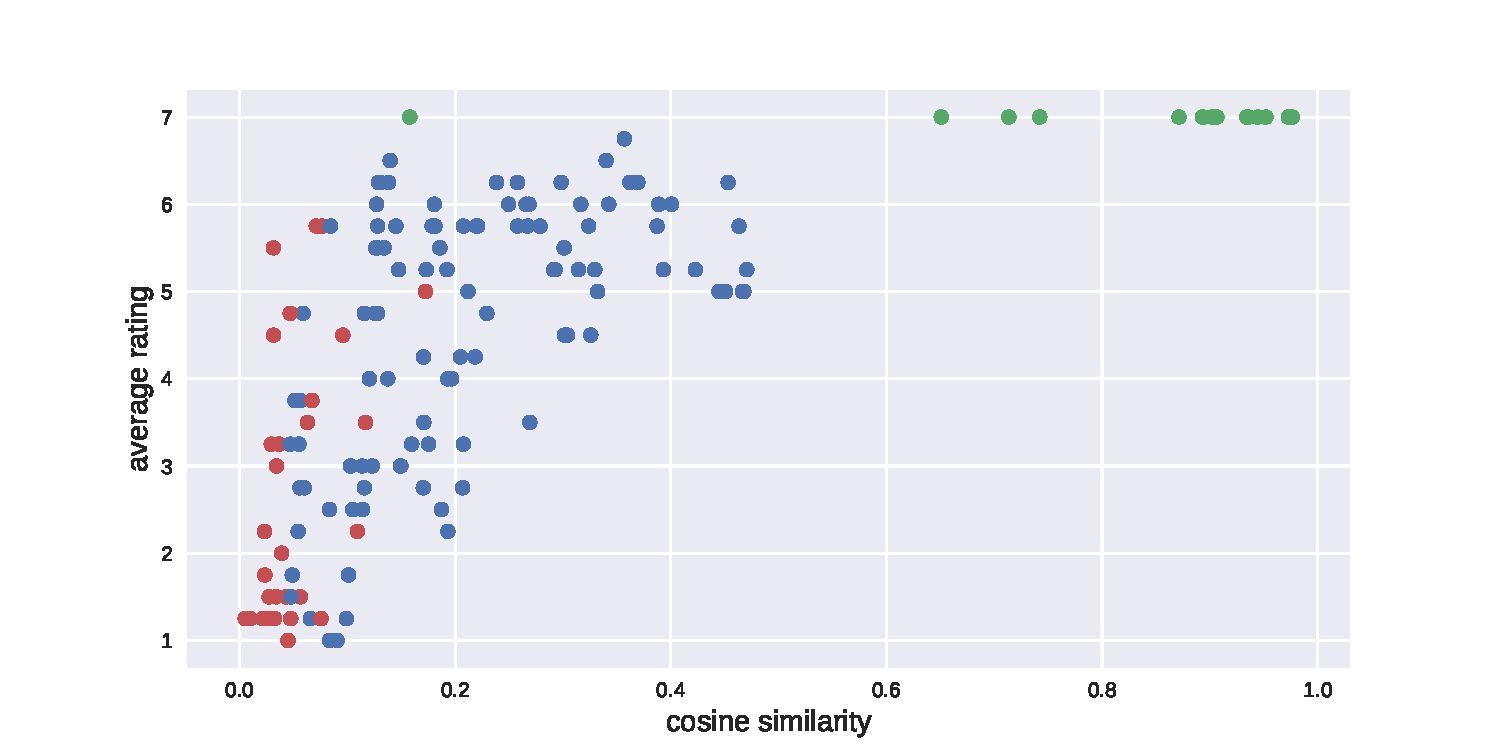
\includegraphics[width=\linewidth]{figures/rating_vs_similarity}
	\caption{Average subject rating versus cosine similarity of all letter pairs. Follow-up pairs are marked green, random ones red.}
	\label{fig:all_points}
\end{figure}


\subsection*{Considerations of Precision and Recall}
We furthermore address precision and recall for our recommender system. Precision and recall are measures of the goodness of an information retrieval system where all documents are binarily classified as either relevant or irrelevant given a current query \citep{Manning2008prerec}. In our case a query is a reference letter and we ask the question of whether a comparison letter is relevant or irrelevant given this reference letter. Precision is then a measure of the correctness of the retrieved results. In probabilistic terms it is the probability that a document is relevant given that it is retrieved $\rm{P}(relevant|retrieved)$. Recall is a measure of completeness of the retrieved results and can be expressed as the probability of being retrieved given that the document is relevant P$(retrieved|relevant)$. Both quantities usually exhibit an inverse relationship. One can trade higher precision for lower recall or vice versa. Note that both precision and recall always lie in $[0,1]$.

\begin{figure}
	\centering
	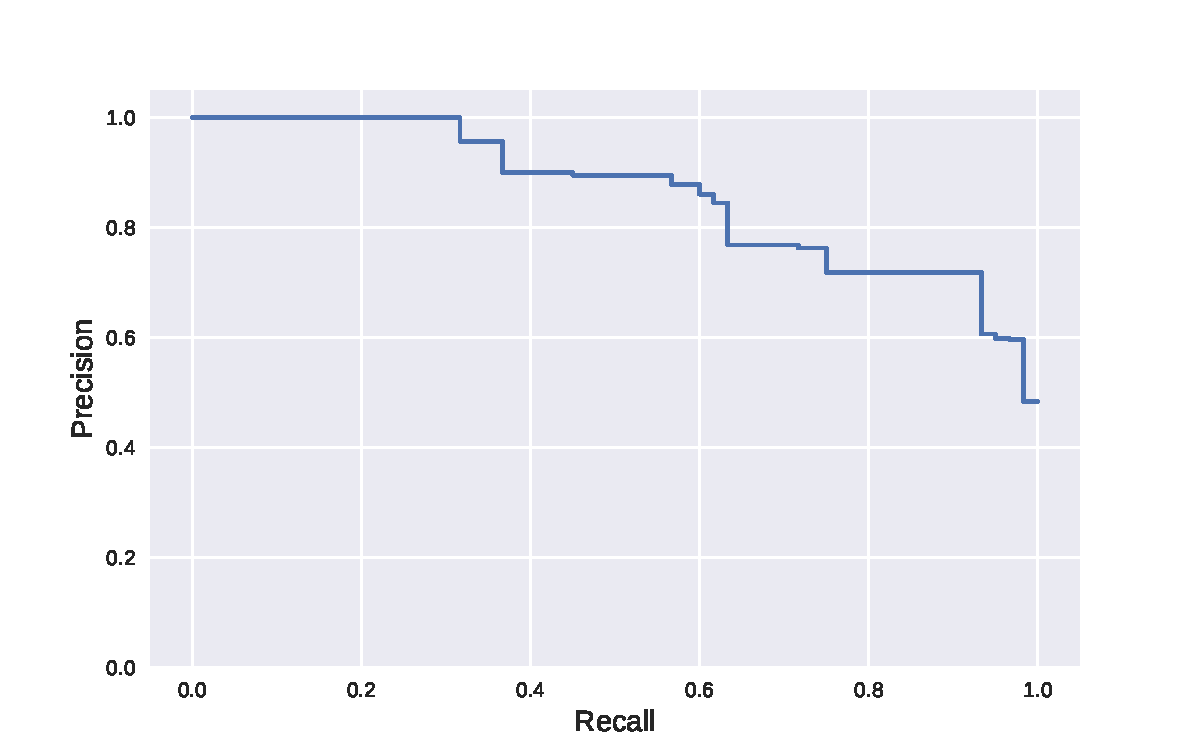
\includegraphics[width=0.7\linewidth]{figures/precision_recall_curve}
	\caption{Precision as a function of recall for letter pairs tested in the experiment.}
	\label{fig:precision_recall_curve}
\end{figure}

The first question we have to consider, when analyzing precision and recall of our system, is asking when a document is considered relevant. We set the threshold for being relevant (somewhat arbitrarily) at an average subject rating of 5 or higher for a given letter pair. That this is a reasonable choice was reinforced through personal discussions with the collaborating doctors. We believe that for the systems use case in a clinic precision is of greater relevance than recall. If doctors are to read the retrieved patient letters regularly in the stressful clinical everyday life, the quality of retrieved results has to be high. This ensures that users find added value in the system and do not discontinue using it because of frustration. If one were using the system for a different purpose, say a research setting in which all patients with similar, extremely rare symptoms are to be found, recall was more important than precision. From figure \ref{fig:all_points} it is now apparent that it is relatively easy to use our system in a way that ensures high precision. If one were for example retrieving only letters with a cosine similarity higher than 0.35, not a single retrieved document would be irrelevant leading to a precision of 1. This comes at the cost of a low recall of 0.25. For a cosine similarity threshold of 0.23, precision is 0.89 and recall 0.57. These numbers have to be taken with a grain of salt. The thresholds were set manually after seeing the data and are therefore overfitted to this particular data. See figure \ref{fig:precision_recall_curve} for a visualization of the interpolated precision recall curve, where one can see all trade-offs between precision and recall. However, these numbers are also somewhat inaccurate. We mainly consider letter pairs found to be among the "best" with our algorithm for this plot. Thereby the selection of pairs is not representative for random samples taken from all possible pairs. Still our sample data covers a wide range of possible cosine similarity values. Therefore we still believe that precision and recall measures as reported here give a useful approximation of the true values.  (!correct! Man könnte den recall über die zufällig ausgewählten pärchen schätzen. In unserem Experiment sind dabei aber 4 von 30 zufälligen relevant, was auf das ganze Datenset gerechnet hieße, dass pro Referenzbrief 40 relevante Briefe vorhanden sind. Das ist aber sicherlich falsch! Und würde auch ganz komische recall zahlen ergeben.)


\subsection*{Considerations for further Work}

We have two additional reasons to believe that our system performs even better in reality than expected from the considerations above. First, when extending our recommender to work on a much larger database, we expect that the best fitting letters to a given reference letter will have much higher cosine similarity, than is the case now. This is because in a much larger database more well fitting documents are expected for each reference letter. For figure \ref{fig:all_points} this means, that we would expect almost no blue points on the left and many more in the region around a cosine similarity of 0.4. These points most likely will be rated highly by subjects, as are all points with such a cosine similarity in our experiment. Second we have reason to believe that some of the letter pairs with low cosine similarity, but high subject rating are due to psychological adjusting. If during one trial only rather badly fitting letters are presented, we believe that subjects adjust their rating scale and rate somewhat fitting letters higher than normally (!correct! Frank nach Paper fragen). Therefore we believe, that getting higher recall might not be as hard as it seems from figure \ref{fig:all_points}.

\begin{figure}
	\centering
	\begin{subfigure}[b]{0.33\textwidth}
		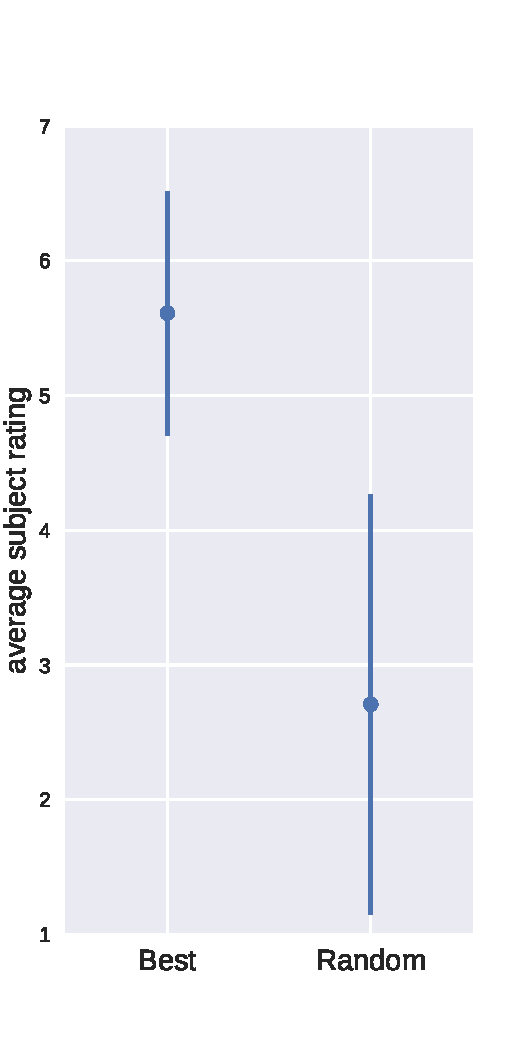
\includegraphics[width=\textwidth, valign=t]{figures/best_vs_random_pv}
		\caption{}
		\label{fig:best_vs_random_pv}
	\end{subfigure}
	\hfill
	\begin{subfigure}[b]{0.66\textwidth}
		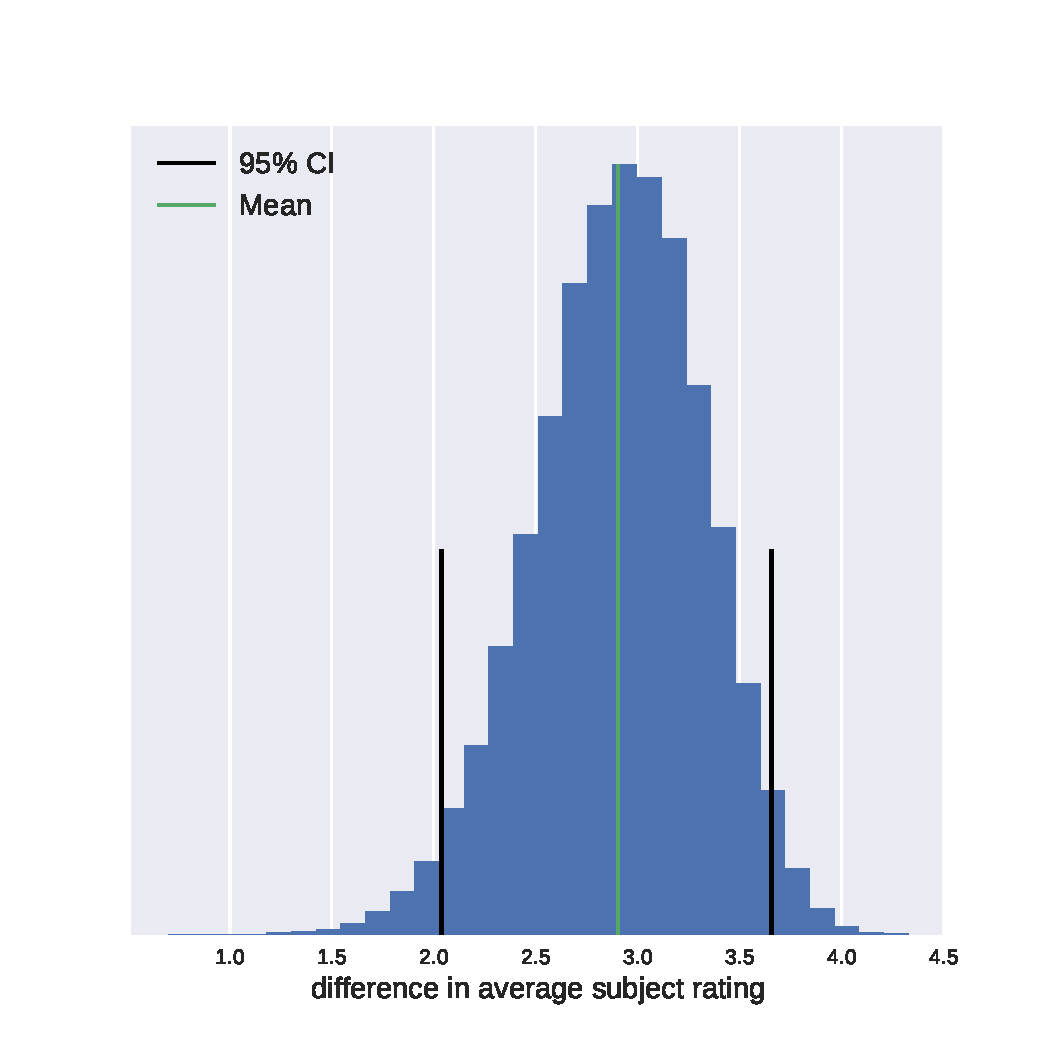
\includegraphics[width=\textwidth, valign=t]{figures/mean_diff_best_random_pv}
		\caption{}
		\label{fig:bootstrap_diff_pv}
	\end{subfigure}
	\caption{\textbf{(a):} Means and standard deviations of averaged subject ratings for the best letters chosen by a combination of tf-idf and paragraph vector embeddings and randomly chosen letters.
		\textbf{(b):} Histogram of the differences in the means of averaged subject ratings of the two groups for 100.000 bootstrap resampled datasets. Black: 95\% Confidence Interval, Green: Mean}	
\end{figure}

Finally one can ask whether there are possibilities to improve the system further. The tf-idf embedding method does not have hyperparameters, so no further tuning of those is possible. We believe, however, that combining similarity measures from several embedding approaches is useful. Of the five embedding methods we tested only paragraph vector is a promising option for improving the results of the retrieval. Bag of words is more or less the simple basis for tf-idf, LSA is highly correlated with tf-idf as it is a feature compressed version of the latter, LDA performed severely worse than all other methods, leaving only paragraph vector. This method performed almost as well as tf-idf during our fine-tuning and computes feature vectors in a very different way, possibly complementing tf-idf well. Indeed we find cues that combining these two methods yields substantially better results. We again compare the mean average subject rating given to letter pairs for two groups. One of the groups consists as above of all the 30 randomly selected letters. The other group consists of the letters from our experimental dataset, that paragraph vector ranks on the first place out of all letters from our complete database. I.e. letters in this group are ranked among the top four by tf-idf and top one by paragraph vector in our whole dataset. We only find 9 of these letters out of the 30 possible trials. Again we look at the differences in mean in figure \ref{fig:best_vs_random_pv} and the distribution of mean differences for 100.000 bootstrap resamples in figure \ref{fig:bootstrap_diff_pv}. Comparing theses with figures \ref{fig:best_vs_random} and \ref{fig:bootstrap_diff}, where only tf-idf information was used, we see that additionalyy using information from the paragraph vector embedding improves results substantially. The mean difference in rating means for example is improved from 1.9 to 2.9 on the rating scale from 1 to 7. We therefore believe that work addressing how to combine information from different embedding methods is a worthwhile task and should be undertaken by further research.
%Combining with Paragraph Vectors seems promising. Paragraph vector computes different, but also very useful features.
%Precision is already very good. And Precision seems to be more important for clinical every day life than recall. Recall might be more important for a research setting, but doctors will be quickly annoyed, if precision is low.
%Additionally we expect that, if we use a bigger database, we will have almost no datapoints in the low cosine similarity region. 
%Points high up-left might be due to subjects adjusting for the very low similarity in one trial, said one doctor.




\end{document}